\chapter{実験}
\label{chap:experiment}
本研究では,第\ref{chap:proposal}章で述べた提案手法の有効性を検証するために,生成クエリネットワークの元論文で使用されているShepard Metzlerデータセットを用いて,評価実験を行った.本章では,行なった実験の内容について説明した後,実験結果について述べていく.最後に実験結果を踏まえた考察を行う.

\section{実験内容}
ここでは,実験の内容について説明する.はじめに評価実験の概要について述べ,次に実験に用いたデータセットについて説明する.最後に実験条件の詳細を述べる.
\subsection{実験概要}
実験では,第\ref{chap:proposal}章で述べた提案内容に基づき,提案手法とベースライン(生成クエリネットワーク)の比較を行う.実験で扱うタスクでは,モデルはまず多数あるシーンの中からランダムにサンプリングされたあるシーン$i$について,いくつかの視点座標と観測画像のペア群$D_i = \left\{ \left( \bm{v _ { i } ^ { k }} , \bm{x _ { i } ^ { k }} \right) \right\} _ { k = 1 } ^ { M }$をコンテキストとして受け取り,さらに別の視点座標$\bm{v_i^q}$をクエリとして入力される.そして,そのクエリに対応する観測画像$\bm{x_i^q}$を予測して出力する,というものである.
仮定するデータの確率的生成過程と学習に用いる目的関数の違いから以下の2種類の方法を比較する.

\begin{description}
\item[提案手法]\mbox{}\\
データの生成過程をFig. \ref{fig:gm_proposal}のように,シーンに依存する確率的な潜在変数$\bm{z_i}$を用いた確率モデルとして定義し,コンテキスト$D_i$を受け取ったときの$\bm{z_i}$の事後分布$p(\bm{z_i} | D_i ; \theta)$を別のパラメータ$\phi$で定義された分布$q(\bm{z_i} | D_i ; \phi)$で近似する.目的関数には,近似分布を使ってサンプリングした$\bm{z_i}$を用いて生成した予測画像の分布の負の対数尤度の期待値(式(\ref{eq:proposal_loss}))を用いる.

\item[ベースライン(生成クエリネットワーク)]\mbox{}\\
データの生成過程をFig. \ref{fig:gm_meta_gqn}のように,シーンに依存し,コンテキスト$D_i$から決定論的に推論される変数$\bm{r_i}$と個別のデータ($\bm{v_i^k}, \bm{x_i^k}$)に依存する確率的な潜在変数$\bm{z_i^k}$を用いた確率モデルとして定義する.目的関数には,$D_i$から決定論的に推論された$\bm{r_i}$と,($\bm{v_i^q}, \bm{r_i}$)から推論された$\bm{z_i^q}$を用いて生成した予測画像の分布の変分下限の期待値(式(\ref{eq:meta_gqn_elbo}))を用いる.ただし,変分下限を計算するために,($\bm{x_i^q}, \bm{v_i^q}, \bm{r_i}$)から$\bm{z_i^q}$を推論する近似分布をさらに定義する.
\end{description}

両手法ともに,確率的なサンプリングを伴い処理は,再パラメータカトリックを用いて計算グラフを保持し,確率的勾配降下法アリゴリズムAdam\cite{Kingma2014}を用いてニューラルネットワークのパラメータを最適化する.

評価時には,以上のように訓練された両手法のモデルを用いて,検証用のデータセットに対して3つのコンテキストが与えられた場合のクエリに対応する観測画像の予測を行い,その予測精度(ここでは,モデルの出力を平均とし,分散を1とした正規分布での負の対数尤度を用いる)を指標として評価を行う.

提案手法では,ベースライン手法の持つ冗長性の解消や,ベースライン手法が決定論的な推論によって無視してしまっているシーン表現の不確実性の考慮などにより,学習の対象となるパラメータ数を削減し,より高速かつ安定に学習が進み,ベースライン手法を上回る精度での予測が行われることが期待される.

\subsection{データセット}
実験では,DeepMind社がインターネット上で公開している生成クエリネットワークの実験用のデータセット\cite{gqn_dataset}のうち,Shepard Metzlerというデータセットを用いる.Shepard Metzlerでは7つのパーツで構成される物体が3次元空間上に存在するようなシーンが200万個用意され,シーンごとに物体のパーツの構成や色が異なっている(Fig. \ref{fig:gqn_flow}参照).データセットはそれぞれのシーンで様々な視点から物体を観測した15枚の64×64ピクセルの画像で構成されている.実験では,このデータセットを9 : 1の割合で訓練用と検証用に分けて使用する.訓練時には,まず200万のシーンの中から1つをランダムにサンプリングし,そのシーン$i$の中からコンテキストとして用いる画像の枚数を$1 \sim 15$の中からランダムに選び,その枚数分の画像をデータセットからランダムに抽出して,$D_i = \left\{ \left( \bm{v _ { i } ^ { k }} , \bm{x _ { i } ^ { k }} \right) \right\} _ { k = 1 } ^ { M }$とする.さらに,残りの画像の中から予測の対象とするものを1つランダムに選び,クエリ($\bm{v_i^q}, \bm{x_i^q}$)として用いる.この操作を毎ステップ行い,そのデータを用いてミニバッチ学習を行う.

\subsection{実験条件}
提案手法とベースライン手法の条件を揃えるために,両者の差分となる部分以外のハイパーパラメータは全て統一して実験を行なった.具体的には,潜在変数の推論を自己回帰モデルで行う際の推論の繰り返しの数は8とし,学習時の目的関数の算出において,生成分布の対数尤度を計算するために用意する正規分布の分散は常に1とする.また,最適化のアルゴリズムにはともにAdam\cite{Kingma2014}を用い,学習率はベースライン手法の元論文\cite{Eslami2018}と同様にした.

\section{実験結果}
ここからは実験結果について述べていく.まず提案手法の結果について定性的な評価を行い,その後ベースライン手法との比較を定量的な指標を用いて行なっていく.
\subsection{提案手法の定性的評価}
Fig. \ref{fig:generation}は検証用データに対して提案手法を用いて画像生成を行なった結果である.一番上の画像が実際のクエリに対応する正解画像で,2段目の画像が左から学習ステップ数1,200,3,100,8,200のときの生成結果,3段目の画像が左から学習ステップ数19,600, 39,900, 253,400のときの生成結果である.図から見て取れるように,学習初期の1,200ステップ時はモノクロの影のような画像しか生成できていなかったが,3,100ステップまで学習が進むと,物体の形状はまだうまく生成できていないものの,画像に色がつき始める.そして,8,200ステップごろには物体の概形を捉えた画像が生成されはじめ,それ以降は学習が進むに連れて鮮明な画像が生成されるようになっている.最後の253,400ステップは一部ぼやけている画像もあるが,多くの生成画像は元画像と見比べても遜色がないほどに鮮明なものとなっている.このように,提案手法は学習が進むにつれて,より正確な予測が行えるようになっていることが定性的に確認できる.

\begin{figure}[tbp]
  \begin{center}
    \begin{tabular}{ccc}
      &
      \begin{minipage}{0.33\linewidth}
        \begin{center}
          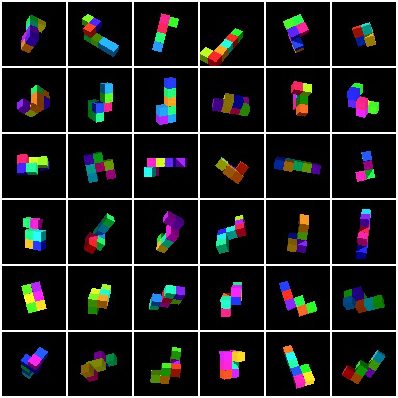
\includegraphics[width=\linewidth]{./figures/groundtruth.png}
        \end{center}
      \end{minipage}
      & \\
      &正解画像&\\
      
      \begin{minipage}{0.33\linewidth}
        \begin{center}
          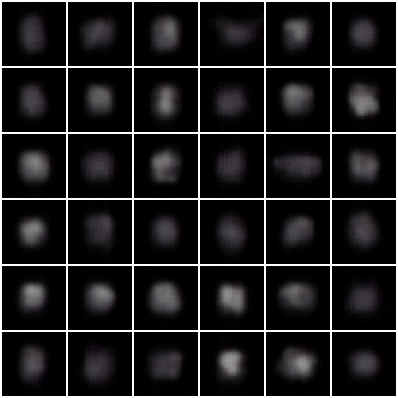
\includegraphics[width=\linewidth]{./figures/proposal1200.png}
        \end{center}
      \end{minipage}&
      \begin{minipage}{0.33\linewidth}
        \begin{center}
          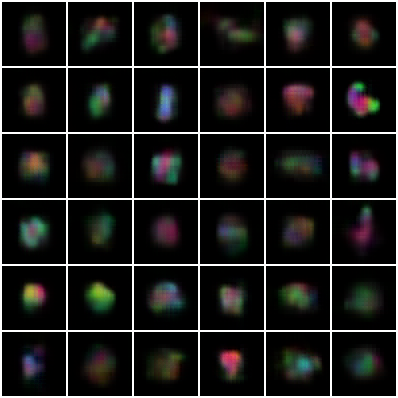
\includegraphics[width=\linewidth]{./figures/proposal3100.png}
        \end{center}
      \end{minipage}&
      \begin{minipage}{0.33\linewidth}
        \begin{center}
          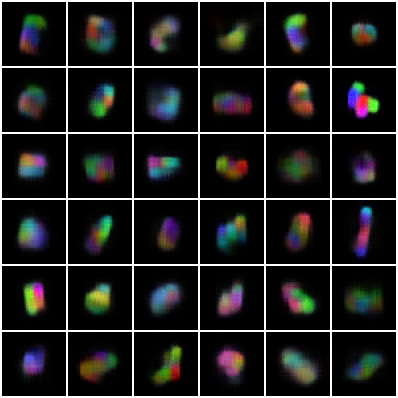
\includegraphics[width=\linewidth]{./figures/proposal8200.png}
        \end{center}
      \end{minipage} \\ 
      1,200ステップ&3,100ステップ&8,200ステップ\\

      \begin{minipage}{0.33\linewidth}
        \begin{center}
          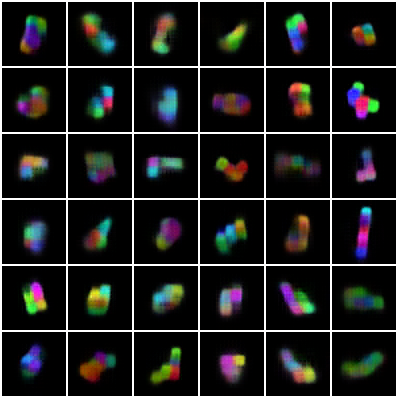
\includegraphics[width=\linewidth]{./figures/proposal19600.png}
        \end{center}
      \end{minipage}&
      \begin{minipage}{0.33\linewidth}
        \begin{center}
          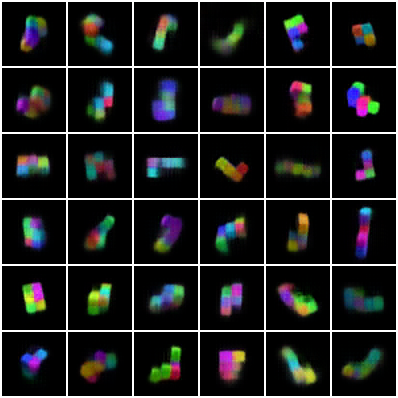
\includegraphics[width=\linewidth]{./figures/proposal39900.png}
        \end{center}
      \end{minipage}&
      \begin{minipage}{0.33\linewidth}
        \begin{center}
          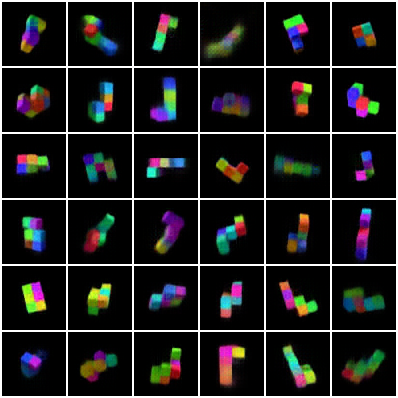
\includegraphics[width=\linewidth]{./figures/proposal253400.png}
        \end{center}
      \end{minipage}\\
      19,600ステップ&39,900ステップ&253,400ステップ
      \end{tabular}
    \caption{学習過程における提案手法による検証用データに対する画像生成結果}
    \label{fig:generation}
  \end{center}
\end{figure}

\subsection{提案手法とベースライン手法の比較}
\subsubsection{定量評価(尤度)}
Fig. \ref{fig:test_loss}は,提案手法とベースライン手法の検証用データに対する予測誤差(負の対数尤度)の推移を示している.青線がベースライン手法,赤線が提案手法の値の推移を表している.図からも明らかなように,ベースライン手法は目的関数に対数尤度に複数の近似を行なった変分下限を用いて,生成分布$p ( \bm{x_i ^ q} | \bm{v_i ^ q} , \bm{z _i^ q} , \bm{r_i} ; \theta )$と2つの近似分布$q(\bm{z_i^q}|\bm{x_i^q}, \bm{v_i^q}, \bm{r_i}; \phi)$, $q^\prime ( \bm{r_i} | D_i ; {\phi}^\prime )$の3つパラメータ$\theta, \phi, \phi^\prime$を同時に最適化しているために,本来最小化すべき予測誤差の推移が学習過程において不安定になってしまっている.一方で,提案手法では必要最低限な推論分布$q ( \bm{z_i} | D_i ; \phi )$の近似のみを行なっているために,安定して予測誤差が減少していることがわかる.

さらにTable \ref{table:evaluation}では,ベースライン手法と提案手法についての定量的な評価指標の値を比較している.負の対数尤度の項は両手法を35,000ステップ学習させたときの検証用データに対する値を表している.負の対数尤度は小さいほど予測誤差が小さいことを表すため,この指標でも提案手法はベースライン手法よりも良い結果を残していることがわかる.

\begin{figure}[tbp]
  \begin{center}
    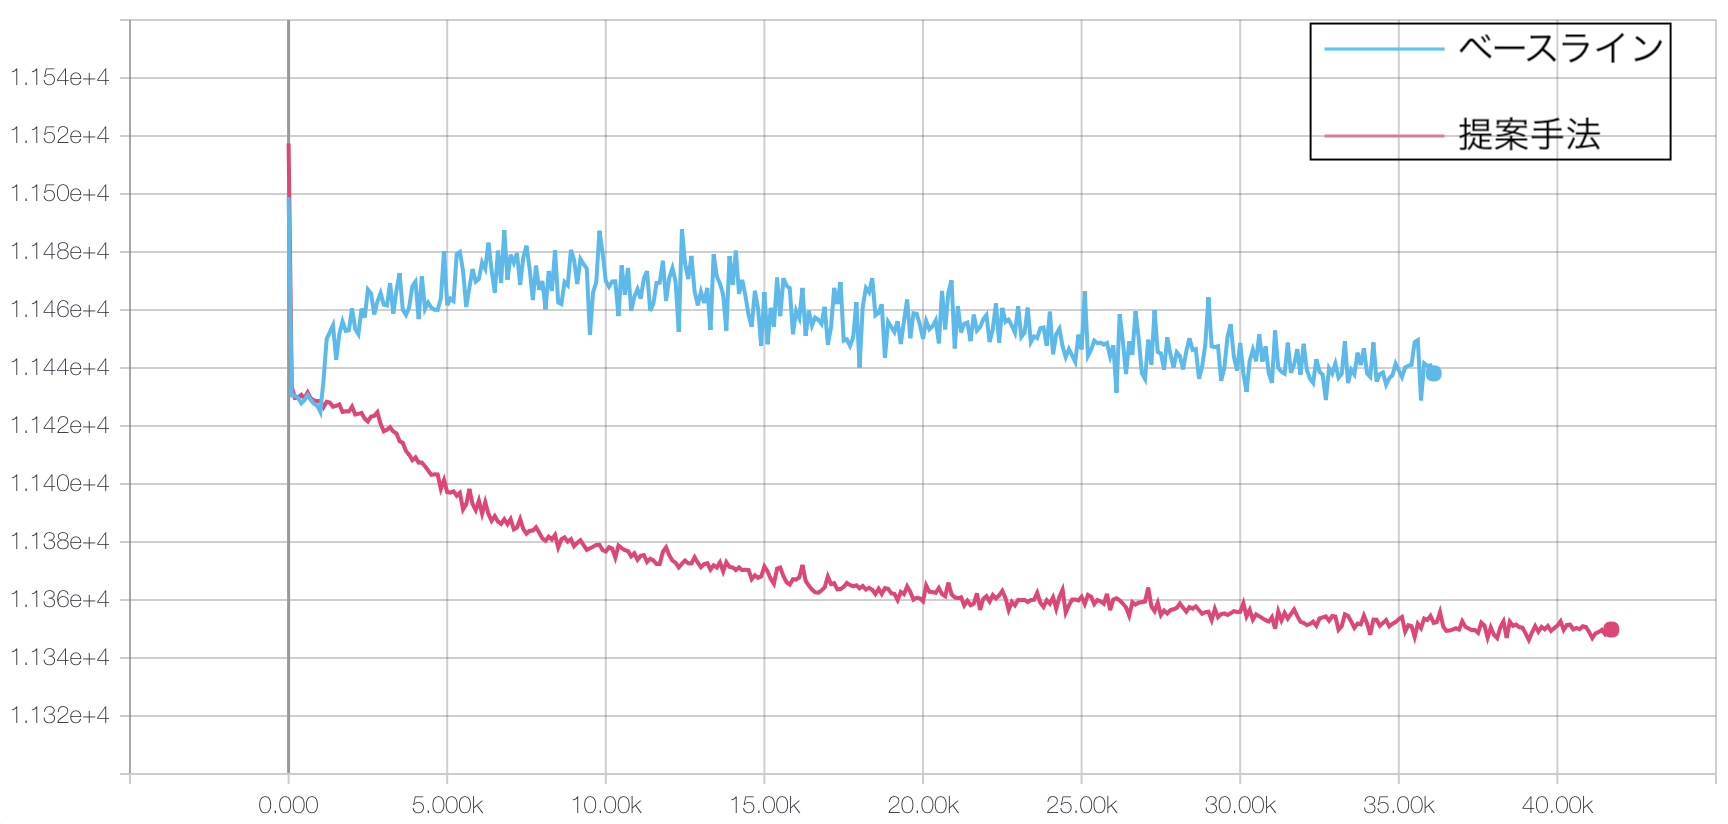
\includegraphics[width=\linewidth]{./figures/test_loss.png}
    \caption{提案手法とベースライン手法の検証用データに対する負の対数尤度の推移}
    横軸はステップ数,縦軸は予測誤差(負の対数尤度)を表す.
    \label{fig:test_loss}
  \end{center}
\end{figure}

\subsubsection{定量評価(パラメータ数)}
Table \ref{table:evaluation}では尤度だけではなく,学習において最適化の対象となるニューラルネットワークのパラメータの総数でも,ベースライン手法と提案手法の比較を行なっている.ベースライン手法では,観測不可能な変数として$\bm{r_i}$と$\bm{z_i^k}$の2つを定義しているために,それらの推論を行う近似分布のモデリングのために,多くのニューラルネットワークを用意する必要があり,その分パラメータ数が増大してしまうが,提案手法では,新たに定義している変数はシーンに固有の潜在変数$\bm{z_i}$のみであるため,ベースライン手法と比較してパラメータ数を削減することができる.実際,Table \ref{table:evaluation}によると,提案手法のパラメータ数はベースライン手法の40\%未満となっており,実験上もパラメータ数の削減が達成できていることがわかる.パラメータ数を減らすことの利点は,最適化が容易になる,計算機リソースが限られるような場合にもモデルの学習を行うことができる,などが挙げられる.特に生成クエリネットワークのような深層生成モデルの場合には,一般に大きなモデルアーキテクチャを使用することが多く,必然的にパラメータ数が増大しやすい傾向にあるため,少ないパラメータで良い精度が得られることは,大きな利点であると言える.多くの場合,パラメータ数を削減することは,モデルの表現力を下げることに相当するため,精度とのトレードオフになるが,今回の場合は,パラメータ数を削減した上で,ベースラインを上回る精度を達成しているため,この結果は提案手法の有効性を強く裏付けていると言える.

\begin{table}[tbp]
  \begin{center}
  \caption{手法ごとの定量評価指標(パラメータ数,尤度)}
  \begin{tabular}{|c||c|c|} \hline
    手法 & パラメータ数 & 負の対数尤度 \\ \hline \hline
    ベースライン & $49,469,343$ & $1.1439 \times 10^4$ \\ \hline
    提案手法 & $\bm{18,713,091}$ & $\bm{1.1353 \times 10^4}$ \\ \hline
  \end{tabular}
  \label{table:evaluation}
  \end{center}
\end{table}

\subsubsection{定性比較}
Fig. \ref{fig:comparison}は学習が35,000ステップ進んだ時点での検証用データに対するベースライン手法と提案手法の生成画像を比較したものである.上段の画像が実際のクエリに対応する正解画像であり,下段の左がベースライン手法の予測,右が提案手法の予測となっている.提案手法は少ない学習時間でもある程度物体の色や形状を正しく捉えた画像が生成できているのに対し,ベースライン手法はこの時点では多くの画像で正しい予測が出来ておらず,一部では物体が分裂したような画像を生成してしまっていることがわかる.

\begin{figure}[tbp]
  \begin{center}
    \begin{tabular}{cc}
      \multicolumn{2}{c}{
      \begin{minipage}{0.5\linewidth}
        \begin{center}
          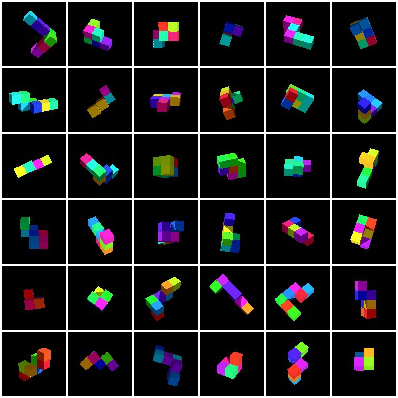
\includegraphics[width=\linewidth]{./figures/comparison_groundtruth.png}
        \end{center}
      \end{minipage} }\\
      \multicolumn{2}{c} {正解画像} \\
      \begin{minipage}{0.5\linewidth}
        \begin{center}
          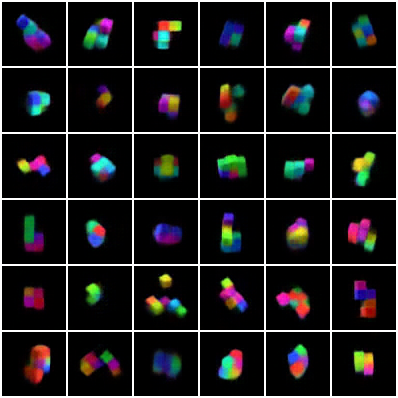
\includegraphics[width=\linewidth]{./figures/comparison_baseline.png}
        \end{center}
      \end{minipage}&
      \begin{minipage}{0.5\linewidth}
        \begin{center}
          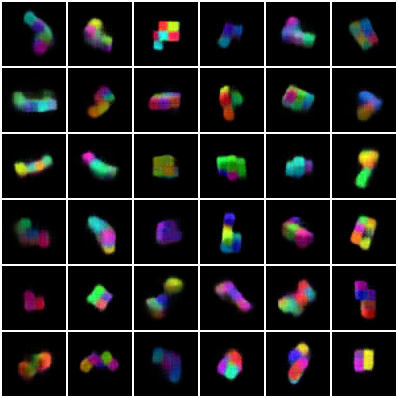
\includegraphics[width=\linewidth]{./figures/comparison_proposal.png}
        \end{center}
      \end{minipage} \\
      ベースライン&提案手法
    \end{tabular}
    \caption{ベースライン手法と提案手法の検証用データに対する画像生成の比較}
    \label{fig:comparison}
  \end{center}
\end{figure}


また,Fig. \ref{fig:comparison_single}では,異なるコンテキスト数でのベースライン手法と提案手法の予測画像の比較を示している.最上段はコンテキストとして与える画像,2段目がクエリに対応する正解画像,3, 4段目がそれぞれベースライン手法と提案手法の予測画像で,コンテキスト数が左から1, 2, 3個の場合の予測を表している.コンテキストが1つの場合,ベースライン手法では物体の形状や色を正しく捉えて生成できていないのに対し,提案手法ではコンテキスト数によらず,正解画像とほとんど見分けがつかないレベルで正しい予測ができていることが見て取れる.

このように,提案手法はベースライン手法と比較して,学習が安定しているために,少ない学習時間でも十分な性能が得られ,さらに予測精度の面でも良い結果が得られることが定性的にも確認できる.

\begin{figure}[tbp]
  \begin{center}
    \begin{tabular}{ccc}
      \begin{minipage}{0.2\linewidth}
        \begin{center}
          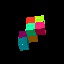
\includegraphics[width=\linewidth]{./figures/context_1.png}
        \end{center}
      \end{minipage} &
      \begin{minipage}{0.2\linewidth}
        \begin{center}
          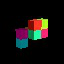
\includegraphics[width=\linewidth]{./figures/context_2.png}
        \end{center}
      \end{minipage} &
      \begin{minipage}{0.2\linewidth}
        \begin{center}
          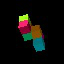
\includegraphics[width=\linewidth]{./figures/context_3.png}
        \end{center}
      \end{minipage} \\
      {\bf コンテキスト1}&{\bf コンテキスト2}&{\bf コンテキスト3}\\
      \multicolumn{3}{c}{
      \begin{minipage}{0.33\linewidth}
        \begin{center}
          
\includegraphics[width=\linewidth]{./figures/ground_truth_single.png}
        \end{center}
      \end{minipage} } \\
      \multicolumn{3}{c} {\bf 正解画像} \\
      コンテキスト数: 1&コンテキスト数: 2&コンテキスト数: 3\\
      \begin{minipage}{0.33\linewidth}
        \begin{center}
          
\includegraphics[width=\linewidth]{./figures/baseline_pred_1.png}
        \end{center}
      \end{minipage} &
      \begin{minipage}{0.33\linewidth}
        \begin{center}
          
\includegraphics[width=\linewidth]{./figures/baseline_pred_2.png}
        \end{center}
      \end{minipage} &
      \begin{minipage}{0.33\linewidth}
        \begin{center}
          
\includegraphics[width=\linewidth]{./figures/baseline_pred_3.png}
        \end{center}
      \end{minipage} \\
      \multicolumn{3}{c} {\bf ベースライン手法} \\
      \begin{minipage}{0.33\linewidth}
        \begin{center}
          
\includegraphics[width=\linewidth]{./figures/proposal_pred_1.png}
        \end{center}
      \end{minipage} &
      \begin{minipage}{0.33\linewidth}
        \begin{center}
          
\includegraphics[width=\linewidth]{./figures/proposal_pred_2.png}
        \end{center}
      \end{minipage} &
      \begin{minipage}{0.33\linewidth}
        \begin{center}
          
\includegraphics[width=\linewidth]{./figures/proposal_pred_3.png}
        \end{center}
      \end{minipage} \\
      \multicolumn{3}{c} {\bf 提案手法} \\
    \end{tabular}
    \caption{異なるコンテキスト数でのベースライン手法と提案手法の予測画像例}
    \label{fig:comparison_single}
  \end{center}
\end{figure}

\subsection{ハイパーパラメータへの頑健性}
最後に,各手法のハイパーパラメータへの頑健性について比較する.ここでは,両手法の潜在変数$\bm{z}$のチャンネル数を3通り(3, 32, 128)に変化させた場合に,学習やモデルの性能に与える影響について検証する.この実験では,それぞれの場合について1万ステップの学習を行い,学習過程における予測誤差の推移を比較することで,その影響について考察を行う.

Fig. \ref{fig:comparizon_z}がその結果である.ただし,凡例の括弧内の数字は潜在変数のチャンネル数を表す.ベースライン手法では,潜在変数のチャンネル数によって結果が大きく変化しており,特にチャンネル数が128の場合には,学習の初期段階から予測誤差の改善が見られなくなっていることがわかる.これは,ベースライン手法では,潜在変数$\bm{z_i^q}$のサンプリングを近似分布$q(\bm{z_i^q}|\bm{x_i^q}, \bm{v_i^q}, \bm{r_i}; \phi)$から行なっており,パラメータの更新に用いる式(\ref{eq:meta_gqn_elbo})の目的関数では,その近似分布を$p ( \bm{x_i ^ q} | \bm{v_i ^ q} , \bm{z _i^ q} , \bm{r_i} ; \theta )$に対して近づけるカルバックライバー距離の項が存在するため,$\bm{z_i^q}$の次元数(チャンネル数)が大きくなった場合に,この項を過剰に最小化する局所解に陥り,学習がうまく進まなくなってしまうことが原因として考えられる.

一方で,提案手法の目的関数には,潜在変数$\bm{z_i}$の確率分布間の距離を測る項が存在しないため,潜在変数の次元数の変化に対して頑健であり,実際にどのチャンネル数の場合にもうまく学習が進んでいることがわかる.一般に,潜在変数の次元数が大きいほど,モデルの表現力は高いと言えるため,その値に対して学習が安定していることは,モデルの性能を容易にチューニングすることを可能にするため,モデルの適用範囲を広げることに繋がり,より汎用的なモデルの構築が可能になったと言うことができる.

\begin{figure}[tbp]
  \begin{center}
    \includegraphics[width=\linewidth]{./figures/comparison_z.png}
    \caption{潜在変数のチャンネル数が変化した場合の提案手法とベースライン手法の検証用データに対する負の対数尤度の推移}
   \end{center}
    横軸はステップ数,縦軸は予測誤差(負の対数尤度)を表す.凡例の括弧内の数字は潜在変数のチャンネル数を示している.
    \label{fig:comparizon_z}
\end{figure}

\section{結果の考察}
評価実験を通じて,提案手法がベースライン手法と比較して,少ないパラメータで安定して学習が進み,未知の視点からの観測画像の予測をより高精度に行えることを定性的・定量的に示した.

特に,生成画像の予測誤差(負の対数尤度)の推移では,ベースライン手法と顕著な差が出ており,提案手法の有効性を裏付ける結果となった.ベースライン手法が学習初期の段階で予測誤差が増加(尤度が減少)してしまっているのは,本来最大化したいはずの対数尤度について,2つの近似分布を導入した変分下限をとって最適化してしまっていることが原因で生じる現象であると考えられる.つまり,ベースライン手法が最適化に用いる式(\ref{eq:meta_gqn_elbo})では,第1項は画像を再構成したときの対数尤度を最大化し,第2項は2つの分布$q(\bm{z_i^q}|\bm{x_i^q}, \bm{v_i^q}, \bm{r_i}; \phi)$と$\pi (\bm{z_i^q} | \bm{v_i^q}, \bm{r_i}; \theta)$のカルバックライブラー距離を最小化するが,\ref{section:interpretation}節で検証したように,$\pi$はすでに分布を決定論的に近似した変数$\bm{r_i}$で条件づけられた分布であり,$q$はさらにその事後分布をもう一度別のパラメータ$\phi$を用いて近似しているため,二重に近似を重ねる形となり,それらの近似を行うパラメータを全て1つ目的関数を用いて同時に最適化する必要があるため,学習が不安定になっているということが実験的にも検証できていると言える.一方で,提案手法では,常に尤度を増加(負の対数尤度を減少)する方向に推移しており,高速かつ安定な学習が行われていることがわかる.これは,ベースライン手法の冗長性を排除した結果,1つの近似分布$q(\bm{z_i}|D_i:\phi)$のみを用いて,真の尤度のより良い近似値を最大化するように学習を行えるようになったからであると考えられる.また,このような冗長性を排除したモデル設計により,潜在変数の次元数のハイパーパラメータに対しても非常に頑健なモデルとなっており,モデルの適用範囲を拡大することが容易となったことが実験的にも示された.

このように,生成クエリネットワークの問題点として挙げられていた学習の不安定性,パラメータ数の膨大さ,ハイパーパラメータへの頑健性は,提案手法によって大きく改善されたことが評価実験を通して確認された.